\documentclass{beamer}

\usepackage[utf8]{inputenc}
\usepackage{textcomp}
\usepackage[official]{eurosym}
\usepackage[polish]{babel}
\usepackage{amsthm}
\usepackage{graphicx}
\usepackage[T1]{fontenc}
\usepackage{scrextend}
\usepackage{hyperref}
\usepackage{xcolor}
\usepackage{listings}
\graphicspath{ {./fig/} }

\usetheme{default}
\usecolortheme{seahorse}

\title{Viua VM w akcji}
%%\subtitle{Implementacja wysokopoziomowego języka programowania i realizacja prostej aplikacji}
\subtitle{Implementacja wysokopoziomowego języka programowania i realizacja prostej aplikacji
\\
\emph{Viua VM in action. Implementation of a high-level programming language and a simple application}}
\author{Marek Marecki \and Krzysztof Franek}

\begin{document}
\lstset{basicstyle=\ttfamily\color{black},
columns=fixed,
escapeinside={\%*}{*)},
inputencoding=utf8,
extendedchars=true,
moredelim=**[is][\color{red}]{@}{@}}

%% PLAN PREZENTACJI
%%
%% Powinniśmy się zamknąć w maksimum 15 slajdach.
%%
%% 00. slajd tytułowy
%%
%% 01. początki Viua VM
%% 02. podział pracy w projekcie
%%
%% 03. o języku (elementy)
%% 04. ciekawostka: aktory
%% 05. przykład składni (wszystkie elementy języka w jednej funkcji); wiele slajdów "fizycznych", ale jeden
%%     "logiczny", bo na każdym fizycznym to samo tylko inny element podkreślony kolorem
%% 06. o kompilatorze (fazy, elementy)
%% 07. ciekawostka: analiza składniowa (tokeny fantomowe, pierwszy token decyduje)
%%
%% 08. o czacie
%% 09. ...
%% 10. ...
%% 11. ...
%% 12. ...
%% 13. ???
%% 14. profit!
%%

\frame{\titlepage}

\begin{frame}
    \frametitle{Viua VM -- tytułem wstępu}

    Viua VM to projekt rozpoczęty w połowie grudnia 2014.

    ~\\

    Jest to maszyna wirtualna wykorzystująca model aktorów jako główny model przetwarzania.
    Możliwe jest jej programowanie w języku assemblera, a programy są sekwencjami instrukcji modyfikujących
    stan zestawu rejestrów oferowanego przez ISA maszyny.

    ~\\

    Projekt jest udostępniany na licencji GNU GPL v3.
\end{frame}

\begin{frame}
    \frametitle{Zakres pracy inżynierskiej}
    \framesubtitle{Podział zadań}

    Marek Marecki:
    \begin{enumerate}
        \item specyfikacja języka programowania ViuAct
        \item implementacja kompilatora języka ViuAct
    \end{enumerate}

    ~\\

    Krzysztof Franek:
    \begin{enumerate}
        \item specyfikacja wymagań dla programu ViuaChat
        \item implementacja programu ViuaChat w języku ViuAct
    \end{enumerate}
\end{frame}

\begin{frame}
    \frametitle{ViuAct}
    \framesubtitle{Krótko o języku}

    Język ViuAct zapewnia dostęp do większości mechanizmów oferowanych przez Viua VM.

    ~\\

    Jest językiem opartym na wyrażeniach (większość konstrukcji to wyrażenia), ze składnią podobną do Lispa.
    Programy pisane w ViuAct składają się z funkcji porozmieszczanych w modułach.

    ~\\

    Model wykonywania programów jest wzorowany na modelu aktorów.
\end{frame}

\begin{frame}[fragile]
    \frametitle{Przykład kodu}
    \framesubtitle{Wszystkie konstrukcje w ViuAct}

    \begin{small}
    \begin{lstlisting}
(let countdown (n) {
    (let x (try (Std.Actor.receive 1s) (
        (catch Exception _
            (tailcall countdown n)))))

    (let wrapped (struct))
    (:= wrapped.value x)
    (:= wrapped.sequence (Std.copy n))
    (actor f wrapped)

    (if (= n 0) 0 (tailcall countdown (- n 1)))
})
    \end{lstlisting}
    \end{small}
\end{frame}

\begin{frame}[fragile]
    \frametitle{Przykład kodu}
    \framesubtitle{Nazwa i parametry formalne}

    \begin{small}
    \begin{lstlisting}
(let @countdown@ (@n@) {
    (let x (try (Std.Actor.receive 1s) (
        (catch Exception _
            (tailcall countdown n)))))

    (let wrapped (struct))
    (:= wrapped.value x)
    (:= wrapped.sequence (Std.copy n))
    (actor f wrapped)

    (if (= n 0) 0 (tailcall countdown (- n 1)))
})
    \end{lstlisting}
    \end{small}
\end{frame}

\begin{frame}[fragile]
    \frametitle{Przykład kodu}
    \framesubtitle{Ciało funkcji}

    \begin{small}
    \begin{lstlisting}
(let countdown (n) @{
    (let x (try (Std.Actor.receive 1s) (
        (catch Exception _
            (tailcall countdown n)))))

    (let wrapped (struct))
    (:= wrapped.value x)
    (:= wrapped.sequence (Std.copy n))
    (actor f wrapped)

    (if (= n 0) 0 (tailcall countdown (- n 1)))
}@)
    \end{lstlisting}
    \end{small}
\end{frame}

\begin{frame}[fragile]
    \frametitle{Przykład kodu}
    \framesubtitle{Odebranie wiadomości (wywołanie funkcji z modułu)}

    \begin{small}
    \begin{lstlisting}
(let countdown (n) {
    (let x (try (@Std.Actor.receive 1s@) (
        (catch Exception _
            (tailcall countdown n)))))

    (let wrapped (struct))
    (:= wrapped.value x)
    (:= wrapped.sequence (Std.copy n))
    (actor f wrapped)

    (if (= n 0) 0 (tailcall countdown (- n 1)))
})
    \end{lstlisting}
    \end{small}
\end{frame}

\begin{frame}[fragile]
    \frametitle{Przykład kodu}
    \framesubtitle{Obsługa wyjątków (słowa kluczowe)}

    \begin{small}
    \begin{lstlisting}
(let countdown (n) {
    (let x (@try@ (Std.Actor.receive 1s) (
        (@catch@ Exception _
            (tailcall countdown n)))))

    (let wrapped (struct))
    (:= wrapped.value x)
    (:= wrapped.sequence (Std.copy n))
    (actor f wrapped)

    (if (= n 0) 0 (tailcall countdown (- n 1)))
})
    \end{lstlisting}
    \end{small}
\end{frame}

\begin{frame}[fragile]
    \frametitle{Przykład kodu}
    \framesubtitle{Obsługa wyjątków (wyrażenie chronione)}

    \begin{small}
    \begin{lstlisting}
(let countdown (n) {
    (let x (try (@Std.Actor.receive 1s@) (
        (catch Exception _
            (tailcall countdown n)))))

    (let wrapped (struct))
    (:= wrapped.value x)
    (:= wrapped.sequence (Std.copy n))
    (actor f wrapped)

    (if (= n 0) 0 (tailcall countdown (- n 1)))
})
    \end{lstlisting}
    \end{small}
\end{frame}

\begin{frame}[fragile]
    \frametitle{Przykład kodu}
    \framesubtitle{Obsługa wyjątków (wyłapanie wyjątku)}

    \begin{small}
    \begin{lstlisting}
(let countdown (n) {
    (let x (try (Std.Actor.receive 1s) (
        @(catch Exception _@
            (tailcall countdown n)@)@)))

    (let wrapped (struct))
    (:= wrapped.value x)
    (:= wrapped.sequence (Std.copy n))
    (actor f wrapped)

    (if (= n 0) 0 (tailcall countdown (- n 1)))
})
    \end{lstlisting}
    \end{small}
\end{frame}

\begin{frame}[fragile]
    \frametitle{Przykład kodu}
    \framesubtitle{Obsługa wyjątków (wyrażenia obsługi)}

    \begin{small}
    \begin{lstlisting}
(let countdown (n) {
    (let x (try (Std.Actor.receive 1s) (
        (catch Exception _
            (@tailcall countdown n@)))))

    (let wrapped (struct))
    (:= wrapped.value x)
    (:= wrapped.sequence (Std.copy n))
    (actor f wrapped)

    (if (= n 0) 0 (tailcall countdown (- n 1)))
})
    \end{lstlisting}
    \end{small}
\end{frame}

\begin{frame}[fragile]
    \frametitle{Przykład kodu}
    \framesubtitle{\emph{let-binding} (dowiązanie zmiennej)}

    \begin{small}
    \begin{lstlisting}
(let countdown (n) {
    (let x (try (Std.Actor.receive 1s) (
        (catch Exception _
            (tailcall countdown n)))))

    (@let wrapped (struct)@)
    (:= wrapped.value x)
    (:= wrapped.sequence (Std.copy n))
    (actor f wrapped)

    (if (= n 0) 0 (tailcall countdown (- n 1)))
})
    \end{lstlisting}
    \end{small}
\end{frame}

\begin{frame}[fragile]
    \frametitle{Przykład kodu}
    \framesubtitle{Konstruktor \emph{\texttt{struct}}}

    \begin{small}
    \begin{lstlisting}
(let countdown (n) {
    (let x (try (Std.Actor.receive 1s) (
        (catch Exception _
            (tailcall countdown n)))))

    (let wrapped (@struct@))
    (:= wrapped.value x)
    (:= wrapped.sequence (Std.copy n))
    (actor f wrapped)

    (if (= n 0) 0 (tailcall countdown (- n 1)))
})
    \end{lstlisting}
    \end{small}
\end{frame}

\begin{frame}[fragile]
    \frametitle{Przykład kodu}
    \framesubtitle{Przypisanie do pola struktury}

    \begin{small}
    \begin{lstlisting}
(let countdown (n) {
    (let x (try (Std.Actor.receive 1s) (
        (catch Exception _
            (tailcall countdown n)))))

    (let wrapped (struct))
    (@:= wrapped.value x@)
    (:= wrapped.sequence (Std.copy n))
    (actor f wrapped)

    (if (= n 0) 0 (tailcall countdown (- n 1)))
})
    \end{lstlisting}
    \end{small}
\end{frame}

\begin{frame}[fragile]
    \frametitle{Przykład kodu}
    \framesubtitle{Wywołanie aktora}

    \begin{small}
    \begin{lstlisting}
(let countdown (n) {
    (let x (try (Std.Actor.receive 1s) (
        (catch Exception _
            (tailcall countdown n)))))

    (let wrapped (struct))
    (:= wrapped.value x)
    (:= wrapped.sequence (Std.copy n))
    (@actor@ f wrapped)

    (if (= n 0) 0 (tailcall countdown (- n 1)))
})
    \end{lstlisting}
    \end{small}
\end{frame}

\begin{frame}[fragile]
    \frametitle{Przykład kodu}
    \framesubtitle{Konstrukcja warunkowa}

    \begin{small}
    \begin{lstlisting}
(let countdown (n) {
    (let x (try (Std.Actor.receive 1s) (
        (catch Exception _
            (tailcall countdown n)))))

    (let wrapped (struct))
    (:= wrapped.value x)
    (:= wrapped.sequence (Std.copy n))
    (actor f wrapped)

    (@if (= n 0) 0 (tailcall countdown (- n 1))@)
})
    \end{lstlisting}
    \end{small}
\end{frame}

\begin{frame}[fragile]
    \frametitle{Przykład kodu}
    \framesubtitle{Konstrukcja warunkowa (wyrażenie sprawdzane; wywołanie operatora)}

    \begin{small}
    \begin{lstlisting}
(let countdown (n) {
    (let x (try (Std.Actor.receive 1s) (
        (catch Exception _
            (tailcall countdown n)))))

    (let wrapped (struct))
    (:= wrapped.value x)
    (:= wrapped.sequence (Std.copy n))
    (actor f wrapped)

    (if (@= n 0@) 0 (tailcall countdown (- n 1)))
})
    \end{lstlisting}
    \end{small}
\end{frame}

\begin{frame}[fragile]
    \frametitle{Przykład kodu}
    \framesubtitle{Konstrukcja warunkowa (...jeśli prawda)}

    \begin{small}
    \begin{lstlisting}
(let countdown (n) {
    (let x (try (Std.Actor.receive 1s) (
        (catch Exception _
            (tailcall countdown n)))))

    (let wrapped (struct))
    (:= wrapped.value x)
    (:= wrapped.sequence (Std.copy n))
    (actor f wrapped)

    (if (= n 0) @0@ (tailcall countdown (- n 1)))
})
    \end{lstlisting}
    \end{small}
\end{frame}

\begin{frame}[fragile]
    \frametitle{Przykład kodu}
    \framesubtitle{Konstrukcja warunkowa (...jeśli fałsz)}

    \begin{small}
    \begin{lstlisting}
(let countdown (n) {
    (let x (try (Std.Actor.receive 1s) (
        (catch Exception _
            (tailcall countdown n)))))

    (let wrapped (struct))
    (:= wrapped.value x)
    (:= wrapped.sequence (Std.copy n))
    (actor f wrapped)

    (if (= n 0) 0 (@tailcall countdown (- n 1)@))
})
    \end{lstlisting}
    \end{small}
\end{frame}

\begin{frame}[fragile]
    \frametitle{Przykład kodu}
    \framesubtitle{Wywołanie \emph{tailcall}}

    \begin{small}
    \begin{lstlisting}
(let countdown (n) {
    (let x (try (Std.Actor.receive 1s) (
        (catch Exception _
            (tailcall countdown n)))))

    (let wrapped (struct))
    (:= wrapped.value x)
    (:= wrapped.sequence (Std.copy n))
    (actor f wrapped)

    (if (= n 0) 0 (@tailcall@ countdown (- n 1)))
})
    \end{lstlisting}
    \end{small}
\end{frame}

\begin{frame}
    \frametitle{ViuaChat}
    \framesubtitle{Chat w ViuAct}

    \begin{enumerate}
        \item Prosta aplikacja czatu webowego
        \item Zbudowana w dwóch celach:
        \begin{enumerate}
        	\item Zademonstrowanie możliwości kompilatora
        	\item Przykładowy kod dla przyszłych programistów
        \end{enumerate}
    \end{enumerate}
\end{frame}

\begin{frame}
    \frametitle{ViuaChat}
    \framesubtitle{Metoda wytwórcza}

	,,mini-Scrum''
    \begin{enumerate}
        \item Inspirowany Scumem
        \item Typowe artefakty: \textit{User stories}, backlog, sprinty (1-2 tyg.)
        \item Bez Scrum Mastera
        \item Bez \textit{daily stands}
        \item Kanban via Trello
    \end{enumerate}
\end{frame}

\begin{frame}
    \frametitle{ViuaChat}
    \framesubtitle{Rys funkcjonalności}

    \begin{enumerate}
        \item Możliwość łączenia się z serwerem
        \item Obecność oddzielnych kanałów - pokojów
        \begin{enumerate}
        	\item Mogą dołączać do nich użytkownicy
        	\item Wiadomości wysłane w pokoju są widoczne dla wszystkich użytkowników w nim obecnych
        \end{enumerate}
        \item Możliwość wysyłania prywatnych wiadomości (od użytkownika do użytkownika)
		\item Prymitywny system uprawnień administrator-nieadministrator
		\item Podstawowe narzędzia administracyjne: tworzenie i usuwanie pokojów, wyrzucanie użytkowników z pokojów i z serwera
    \end{enumerate}
\end{frame}

\begin{frame}
    \frametitle{ViuaChat}
    \framesubtitle{Podstawowa architektura}

    \begin{enumerate}
        \item Frontend: Single Page App
        \begin{enumerate}
        	\item Vue.js
        	\item HTML5
        \end{enumerate}
        \item Backend
        \begin{enumerate}
        	\item Serwer Nginx - wystawia statyczny HTML i JS
        	\item Maszyna ViuaVM - właściwy serwer czatu
        \end{enumerate}
        \item Komunikacja front-back: via Websocket
    \end{enumerate}
\end{frame}

\begin{frame}
    \frametitle{ViuaChat}
    \framesubtitle{Diagram komponentów}
	\begin{figure}[!htp]
		\centering
		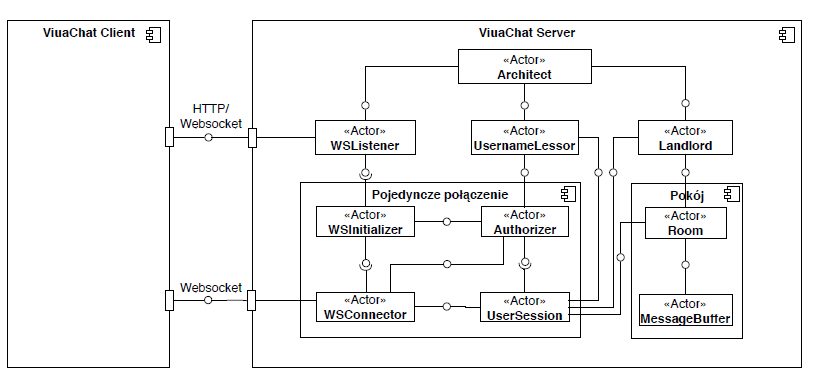
\includegraphics[width=\textwidth]{pckdiag}
		\caption{Diagram komponentów}
		\label{diagram_komponentow}
	\end{figure}
\end{frame}

\begin{frame}
    \frametitle{ViuaVM}
    \framesubtitle{Harmonogram prac}

    \begin{enumerate}
        \item Do końca marca
        \begin{enumerate}
        	\item finalizacja kompilatora ViuAct i specyfikacji ViuaChat
        	\item pierwsza wersja frontendu ViuaChat
        \end{enumerate}         
        \item Do końca kwietnia
        \begin{enumerate}
        	\item finalizacja pierwszej wersji backendu ViuaChat
        	\item pierwsza integracja frontend-backend
        	\item pierwsza wersja \textit{książki} do konsultacji z promotorem
        \end{enumerate}
        \item Do końca maja
        \begin{enumerate}
        	\item realizacja testów stabilności działania ViuaChat
        	\item ukończenie prac nad stabilną wersją ViuaChat
        	\item przygotowanie urządzeń testowych dla zaprezentowania projektu
        	\item ukończenie \textit{książki}
        \end{enumerate}
    \end{enumerate}
\end{frame}


%\begin{frame}
%    \frametitle{ViuaChat}
%    \framesubtitle{Aktory - podstawowe}
%	Są tworzone wraz z inicjalizacją maszyny, występują zawsze w jednym egzemplarzu
%
%    \begin{enumerate}
%    	\item \texttt{Architect} - powstaje jako pierwszy, tworzy pozostałych 3 i pilnuje ich
%        \item \texttt{WSListener} - nasluchuje nowych połączeń od klientów
%        \item \texttt{Landlord} - zarządza pokojami i umożliwia łączenie się z nimi
%        \item \texttt{UsernameLessor} - zarządza nazwami użytkowników i pilnuje, czy nadal są używane
%    \end{enumerate}
%\end{frame}
%
%\begin{frame}
%    \frametitle{ViuaChat}
%    \framesubtitle{Aktory - odpowiedzialne za połączenie}
%	Występuje po jednym zestawie dla każdego otwartego połączenia
%
%    \begin{enumerate}
%    	\item \texttt{WSInitializer} - tworzony natychmiast przez \texttt{WSLister}a; tworzy \texttt{WSConnector}a i \texttt{Authorizer}a po czym ulega samozniszczeniu
%    	\item \texttt{WSConnector} - pośredniczy pomiędzy warstwą WebSocket i wewnętrznym światem serwera (\texttt{Authorizer}em lub \texttt{UserSession})
%        \item \texttt{Authorizer} - próbuje uzyskać nazwę użytkownika, a w razie sukcesu - tworzy \texttt{UserSession} i ulega samozniszczeniu
%        \item \texttt{UserSession} - posiada przypisaną nazwę użytkownika i poziom uprawnień; wysyła/odbiera wiadomości i łączy/rozłącza się z pokojami
%    \end{enumerate}
%\end{frame}
%
%\begin{frame}
%    \frametitle{ViuaChat}
%    \framesubtitle{Aktory - odpowiedzialne za wymianę wiadomości}
%	Występuje po jednym zestawie dla każdego otwartego pokoju
%
%    \begin{enumerate}
%    	\item \texttt{Room} - tworzeni i usuwani przez \texttt{Landlord}a; rozsyłają wiadomości pomiędzy podpięte sesje \texttt{UserSession}
%    	\item \texttt{MessageBuffer} - zapisują ostatnie kilkanaście wiadomości i umożliwiają ich odczytanie w razie potrzeby
%    \end{enumerate}
%\end{frame}


\end{document}
